\documentclass{silreport}

% Document

\begin{document}
\maketitle

% Set 1.5 line spacing for rest of the document
\onehalfspacing

\section*{Abstract}
\addcontentsline{toc}{chapter}{Abstract}
\lipsum[1-2]
\cleardoublepage


\section*{Acknowledgments}
\addcontentsline{toc}{chapter}{Acknowledgments}
\lipsum[1]
\cleardoublepage

% Start : \chapter* redefiniton
% https://tex.stackexchange.com/questions/62125/how-to-remove-top-margin-above-tableofcontents
\begingroup
% Reset to single line spacing for ToC
\singlespacing
\makeatletter
% Redefine the \chapter* header macro to remove vertical space
\def\@makeschapterhead#1{%
  %\vspace*{50\p@}% Remove the vertical space
  {\parindent \z@ \raggedright
    \normalfont
    \interlinepenalty\@M
    \Huge \bfseries  #1\par\nobreak
    \vskip 40\p@
  }}
\makeatother

% Insert contents lists
% Comment if not required
\tableofcontents
\listoffigures
\listoftables
\cleardoublepage
\endgroup
% End : \chapter* redefiniton
  
% Start page numbering
\pagenumbering{arabic}
\setcounter{page}{1}


\chapter{Introduction}
Lorem ipsum dolor sit amet, consectetur adipiscing elit. Proin elementum felis suscipit lacus posuere cursus \cite{aws_sam}. Vestibulum varius sapien id nisl convallis, ac vestibulum arcu elementum. Phasellus sed neque vitae mauris maximus interdum quis nec eros. Duis condimentum mi molestie urna commodo facilisis. In elementum et diam et posuere \cite{Cahn:etal:2015}. Ut sodales blandit purus eget euismod. Cras non posuere quam, a mollis dui. Aliquam nisl est, eleifend vitae nunc congue, congue rhoncus libero. Pellentesque elit diam, mollis ac nisl eget, suscipit tempor quam. Duis pellentesque ornare massa at tempor. Aenean maximus tempor quam nec dictum. In cursus dolor felis, at tincidunt lorem elementum non. Phasellus fermentum enim nibh. Nam efficitur ex odio, id auctor libero facilisis non.

\section{Sub Section}
\lipsum[1]

\begin{table}[hbt]
\centering
\begin{tabular}{ll}
\hline
Area & Count\\
\hline
North & 100\\
South & 200\\
East & 80\\
West & 140\\
\hline
\end{tabular}
\caption{This is a table}
\label{tab:sample}
\end{table}
\lipsum[1-2]

\chapter{State of the art}
\lipsum[1-2]

\begin{figure}[htp]
\centering
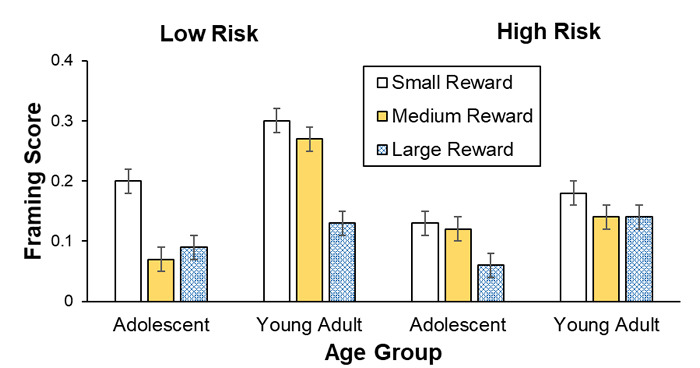
\includegraphics[width=.5\textwidth]{figures/sample_figure.jpg}
\caption{This is a figure}
\label{fig:samplefigure}
\end{figure}

\lipsum[1-2]

\begin{lstlisting}[language=C, caption=Sample C Program, captionpos=b]
  #include <stdio.h>
  int main() {
     // printf() displays the string inside quotation
     printf("Hello World!");
     return 0;
  }
\end{lstlisting}

\lipsum[1-2]



\chapter{Contribution}
\lipsum[1-2]

\begin{figure}
  \centering
      
      \begin{subfigure}{0.5\linewidth}
        \centering
        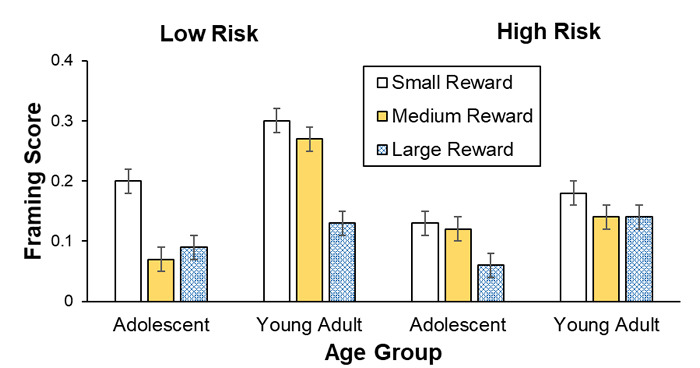
\includegraphics[width=0.5\linewidth]{figures/sample_figure.jpg}
        \caption[Sample short figure (apprears on the ToC)]{Sample long caption.}
        \label{fig:sample_figure_1}
      \end{subfigure}%
      
      \begin{subfigure}{0.5\linewidth}
        \centering
        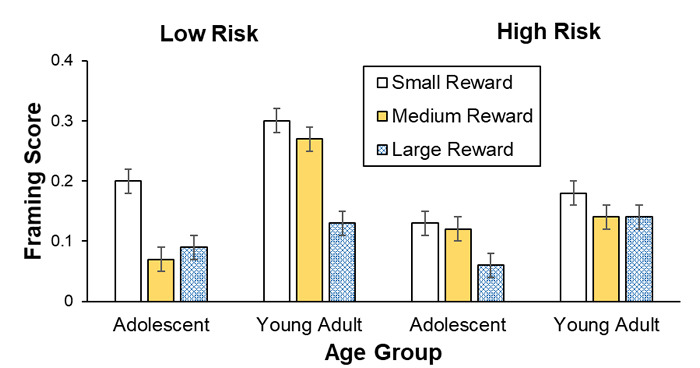
\includegraphics[width=0.5\linewidth]{figures/sample_figure.jpg}
        \caption[Sample short figure (apprears on the ToC)]{Sample long caption.}
        \label{fig:sample_figure_2}
      \end{subfigure}
  
  \caption{Landing page Interactions}
  \label{fig:test}
  \end{figure}
 
  \lipsum[1-2]


\chapter{Conclusion}
\lipsum[1]

% Start : \chapter* redefiniton
% https://tex.stackexchange.com/questions/62125/how-to-remove-top-margin-above-tableofcontents
\begingroup
% Reset to single line spacing for References
\singlespacing
\makeatletter
% Redefine the \chapter* header macro to remove vertical space
\def\@makeschapterhead#1{%
  %\vspace*{50\p@}% Remove the vertical space
  {\parindent \z@ \raggedright
    \normalfont
    \interlinepenalty\@M
    \Huge \bfseries  #1\par\nobreak
    \vskip 40\p@
  }}
\makeatother


\chapter*{References}
\addcontentsline{toc}{chapter}{References}


\begingroup
	\renewcommand{\chapter}[2]{}
  \bibliography{bibliography}	
  \bibliographystyle{ieeetr}
\endgroup


\cleardoublepage
\endgroup
% End : \chapter* redefiniton



%% Appendix : Start %%
%
%\appendix
%\part*{APPENDIX}
%\addcontentsline{toc}{part}{Appendix}
%\cleardoublepage
%
%\chapter{Appendix A}
%
%\cleardoublepage
%\chapter{Appendix B}
%% Appendix : End %%

\cleardoublepage
\end{document}

